%% V1.0
%% by Christopher Leith, udacl@cielsystems.com
%% This is a template for Udacity projects using IEEEtran.cls

\documentclass[10pt,journal,compsoc]{IEEEtran}

\usepackage[pdftex]{graphicx}    
\usepackage{cite}
\hyphenation{op-tical net-works semi-conduc-tor}

\begin{document}

\title{WhereAmI - Robotic Localization}

\author{Christopher Leith}

\markboth{WhereAmI, Localization, Udacity}%
{}
\IEEEtitleabstractindextext{%

\begin{abstract}
In this project we create a simulated robot and demonstrate Adaptive Monte Carlo Localization (AMCL) within the ROS framework to permit navigation within a small simulated "Gazebo" world. A differential drive robot is designed to operate within the Gazebo simulation and uses the ROS navigation stack and the AMCL package for localization within the supplied map. The RViz visualization tool is used to observe the the robot and the relevant paths, maps and point clouds as it moves to a predefined goal. The tuning of configuration parameters of the simulation, navigation stack and AMCL package neccesary for success are discussed.
\end{abstract}

% Note that keywords are not normally used for peerreview papers.
\begin{IEEEkeywords}
Mobile Robot, Localization, Monte Carlo Localiztion, ROS.
\end{IEEEkeywords}}


\maketitle
\IEEEdisplaynontitleabstractindextext
\IEEEpeerreviewmaketitle
\label{sec:Introduction}
\section{Introduction}
\IEEEPARstart{M}{obile} robots must be able to determine their location within their region of operation, a process known as localization, and navigate to other locations reliably in order to perform their tasks succesfully. \hfill \vspace{\baselineskip}

The process of robotic localization requires a known, predefined 'ground truth' map within which the robot, using sensors of various kinds, must establish the exact coordinates, in our case 2D coordinates, of its current location as it moves about the map. The are 3 primary categories of localization, in order of increasing complexity: 'local', 'global' and what is termed 'kidnapped robot' localization.  \hfill \vspace{\baselineskip}

In 'local localization' a robot's position is initially known and the robot must only keep track of its changing location as it moves. In 'global localization' the robot does not initially know its location within the map and must, over time, resolve its location using information from its sensors and the ground truth map. In 'kidnapped robot' localization the robot must always assume that its believed location could be grossly in error and must constantly recalculate its location anew. \hfill \vspace{\baselineskip}

In this project only the simple 'local localization' is demonstrated. That is, the initial location is known accurately and the robot must keep track of its location as it moves.

\section{Background / Formulation}
Because localization is so important for mobile robotics it is a highly researched field and has many well developed techniques and technologies. Most people are familiar with the Global Positioning System (GPS) which permits an electronic device to directly infer its latitude, longitude and altitude based on signals received from GPS satellites. Other techniques such as Kalman filtering and Monte Carlo Localization (aka 'Particle Filter') are techniques that can take input from a variety of sensors and over time compute estimates of the current location. Such sensors include radar, laser scanners, cameras, odometry sensors, Inertial Measurement Units (IMU), sonar, compass sensors and more. In many cases multiple sensor inputs are used simulataneously with theses techniques in a process known as Sensor Fusion. Selecting techniques and sensors is part of the complicated design process of a robot and of course depends on the intended application, the intended environment, eg indoor or outdoor, and the typical engineering constraints of cost, size, power, sensor noise, computational power, and required reliability and performance goals.  \hfill \vspace{\baselineskip}

For this simulation project we are, fortunately, given absolute constraints on all of these design considerations. Specifically the robot is to be a wheeled, differential drive robot operating in a small, flat, 2D environment with only noiseless wheel odometry sensors and a laser scanner and we will discuss only the Kalman filter Monte Carlo Localization techniques and only implement to Monte Carlo technique. Furthermore the application is to occur in a ROS Gazebo simulated environment with a predfined, known 'ground truth' map and a very simple objective of navigating to a predefined goal location.  \hfill \vspace{\baselineskip}

This simple robot objective is, of course, merely a context for the wider objective of learning about techiques and technologies of mobile robotic design. Specifically we are gaining knowledge of the using ROS robotics framework for robotic system design and the the ROS Gazebo simulation environment for development and test and using the ROS Adaptive Monte Carlo Localization (AMCL) package with odometry and laser scanner sensors to learn about important parameter tuning considerations. 

Adaptive Monte Carlo Localization (AMCL) is further discussed below. 
Another powerful localization technique is the Kalman filter. Although the Kalman filter is not used in this project it was used in earlier Lab projects and so it also discussed below.

\subsection{Adaptive Monte Carlo Localization}
The Adaptive Monte Carlo Localization (AMCL) technique, aka 'particle filter', creates a set of hypothetical robot states, or 'particles' distributed at random locations and orientations (aka 'poses' in ROS terminology) around the map. Each of the particles represent a \textit{possible} pose that \textit{ might} correspond to robot's true pose. It then computes the expected laser observations for each of those particles and compares each of those observations against the actual observation and establishes a likelihoood weight for each particle. The likelihood weight represents the degree of correspondence between the particle observation and the actual. The particles with the lowest weights are eliminated from the set of particles. After this the AMCL uses more actual sensor data, in our case the odometry sensors, to update the particle poses to the expected locations due to the movement of the robot. Then the AMCL repeats the process. In this way the algorithm will converge on a set of particles that have a best fit to the actual laser scan observations and either the 'best' particle or an average location of the those best particles will be interpreted as the true location of the robot.
There are many variations of managing the particle set. For example the 'Adaptive' aspect of the AMCL package reduces the total number of particles if the best particles appear to be converging, or adds new particles when the best particles do not appear to correlate well. Another technique is to constantly add new, randomly placed particles to allow the algorithm to 'escape' in the case that it has converged on an incorrect pose, as might easily occur in an environment with a repeating or symetrical spatial features such as a hallway or building with identical rooms even simply in square room with 2 identical doors.
\hfill \vspace{\baselineskip}
The AMCL implementation used in this project is encapsulated in the ROS AMCL package. The AMCL package is closely integrated with ROS navigation stack, specifically with the Move\_base package, the odometry and hokuyo laser scanner system and the tf reference frame transform package. \textbf{ XXX}.

\subsection{Kalman Filter}
Another powerful localization technique is the Kalman filter. Although the Kalman filter is not used in this project it was used in earlier Lab projects. The Kalman filter is an estimation algorithm that treats both the actual state and the observations, from potentially several sensors, as gaussian distributions and combines the two in proportion to the klamn gain which is a value that gives higher weight to quanitities with least uncertainty. As the algorithm iterates it is typically able to converge on a pose with minimal uncertainty.
One of complication of the kalmin filter is that it requires that the error of the sensors be linear and well characterized and be a gaussian distribution. In cases where this does not hold a modified kalman filter, known as the Extended Kalman Filter (EKF), can linearize the uncertainty functions by applying a jacobian transform. This adds complexity to using the kalman filter on some sensors.

\subsection{Monte Carlo vs Kalman Filter}
The MCL techinique is the usual first choice because of its comparitive simplicity and the fact that KF or EKF require knowledge of the sensors uncertainty and that the uncertainties either be a well know, normal distribution and in the cases on non-linearities require more complicated mathematic functions to implemented to linearize it. MCL also can be configured to deal with global localization while EKF can not. On the other hand EKF is more memory and processor efficient so may be worth the extra effort on a smaller computer or if power is a constraint.

\section{Results}
After tuning both models could relaibly navigate to the test goal location.

\subsection{Results: Udacity-Bot}
The Udacity\_bot reliably navigated to the goal in about 90 seconds without any spinning or need for recovery. The initial spread of Monte Carlo particles can be seen in Fig ~\ref{fig:UdaBot Initial Particles}. The converged Monte Carlo particles at the goal can be seen in Fig ~\ref{fig:UdaBot Goal Particles}. The convergence of particles was very rapid: Within seconds of navigation the particles converged to a very accurate estimation of the actual robot pose.

\begin{figure}[h]
      \centering
      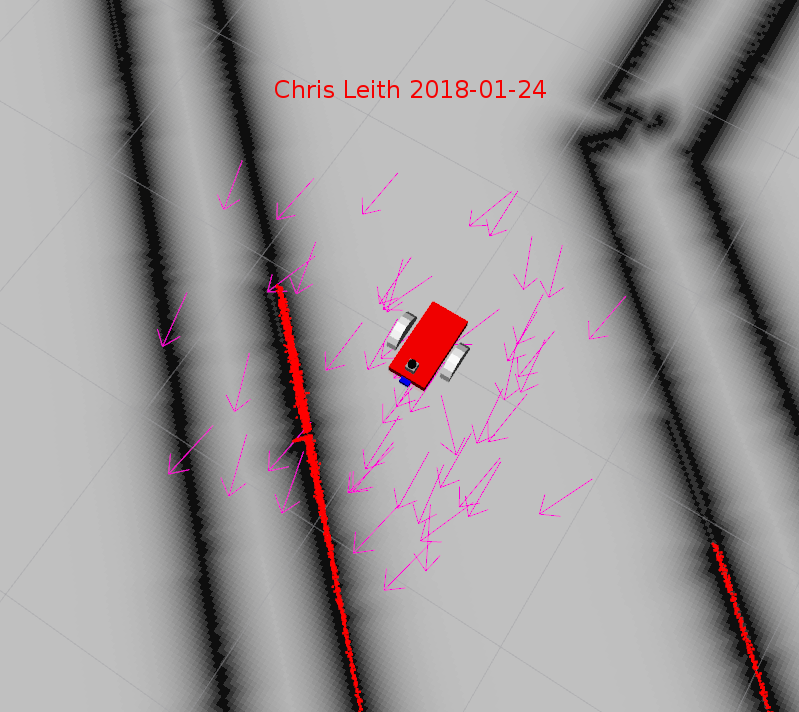
\includegraphics[width=\linewidth]{../Assets/writeupImages/udaBot_rvizInit.png}
      \caption{UdaBot Initial Particles }
      \label{fig:UdaBot Initial Particles}
\end{figure}

\begin{figure}[h]
      \centering
      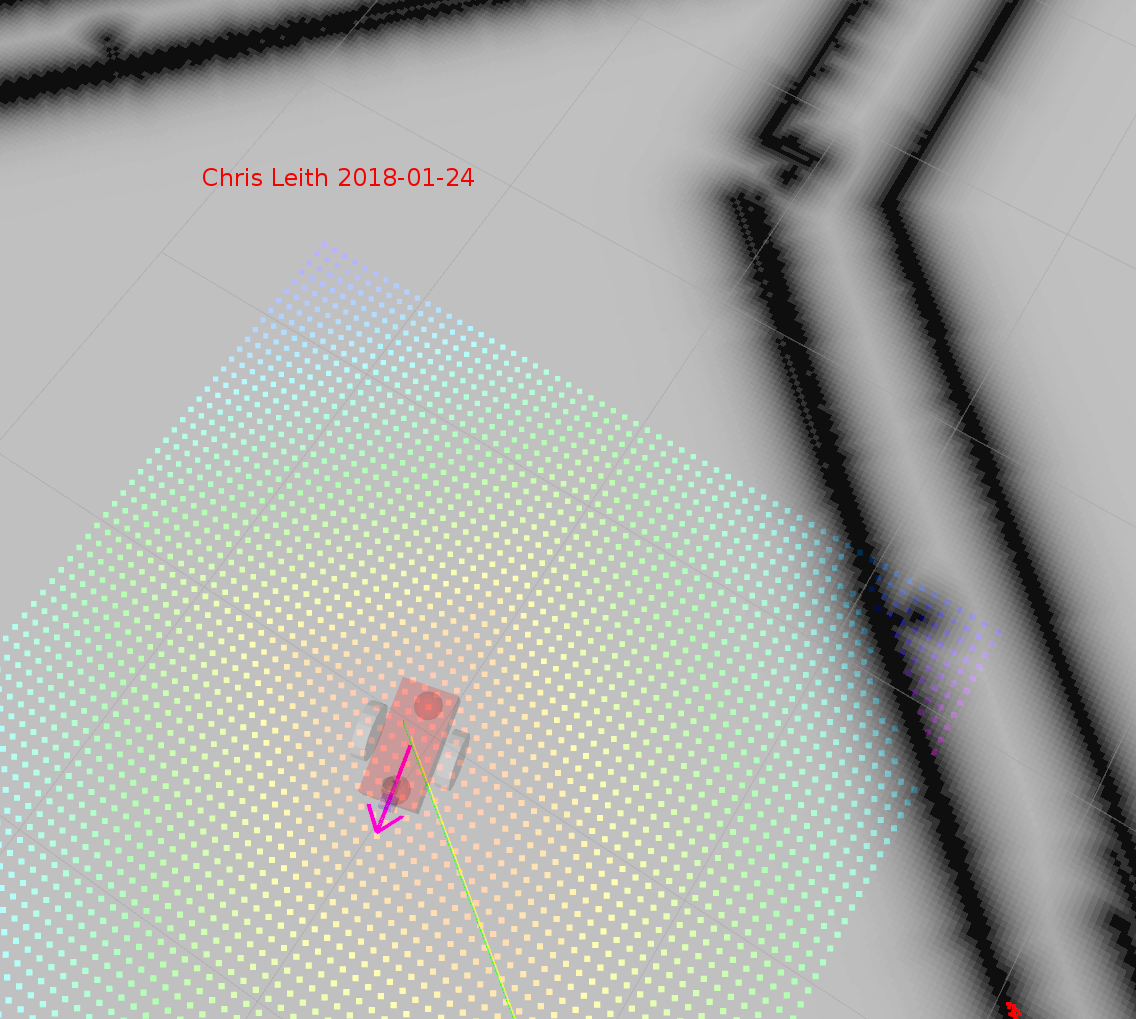
\includegraphics[width=\linewidth]{../Assets/writeupImages/udaBot_rvizGoal.png}
      \caption{UdaBot Goal Particles }
      \label{fig:UdaBot Goal Particles}
\end{figure}

\subsection{Results: Ciel-Bot}
The custom Ciel\_bot reliably navigated to the goal in about 100 seconds without any spinning or need for recovery. Since the design is so similar to the udacity bot the same tuning parameters were used. Concern that the obstruction inflation parameter would need to increase because of the wider wheel base was proven unfounded - it seemed to cut close as it rounded the obstruction but it did not get hung up.
The initial spread of Monte Carlo particles can be seen in Fig ~\ref{fig:cielBot Goal Particles}. 
It is noted that randomization of the initial particles matches exactly those in the seen with the udacity\_bot, which would suggest that the randomization seed is always the same by default, which would make sense when doing testing on robots. As with the udacity bot the particles converged very quickly, in seconds, to a seemingly single particle.

The final, converged Monte Carlo particles at the goal can be seen in Fig ~\ref{fig:cielBot Goal Particles}.

\begin{figure}[h]
      \centering
      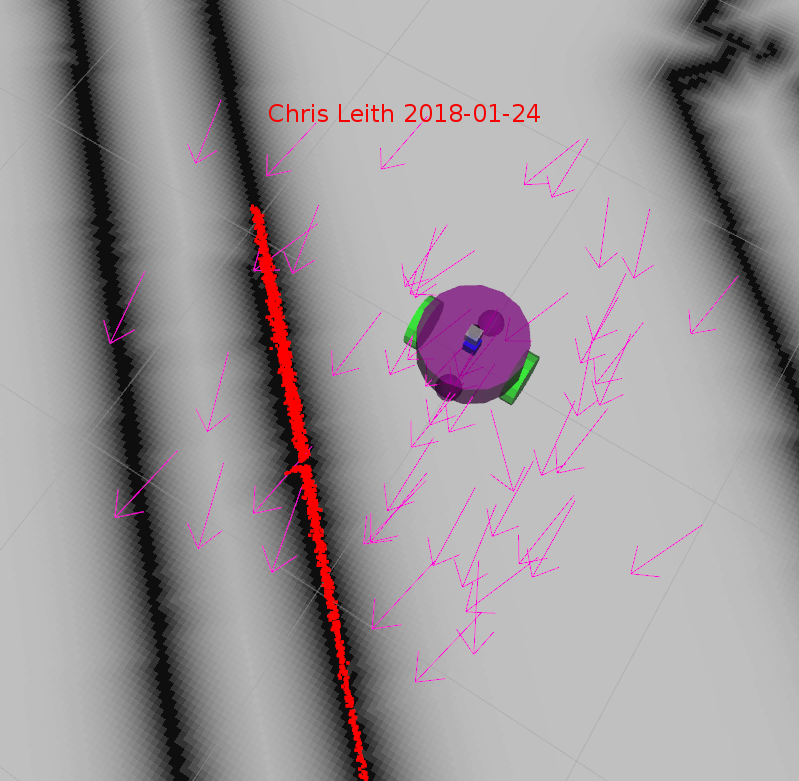
\includegraphics[width=\linewidth]{../Assets/writeupImages/cielBot_rvizInit.png}
      \caption{cielBot Initial Particles }
      \label{fig:cielBot Initial Particles}
\end{figure}

\begin{figure}[h]
      \centering
      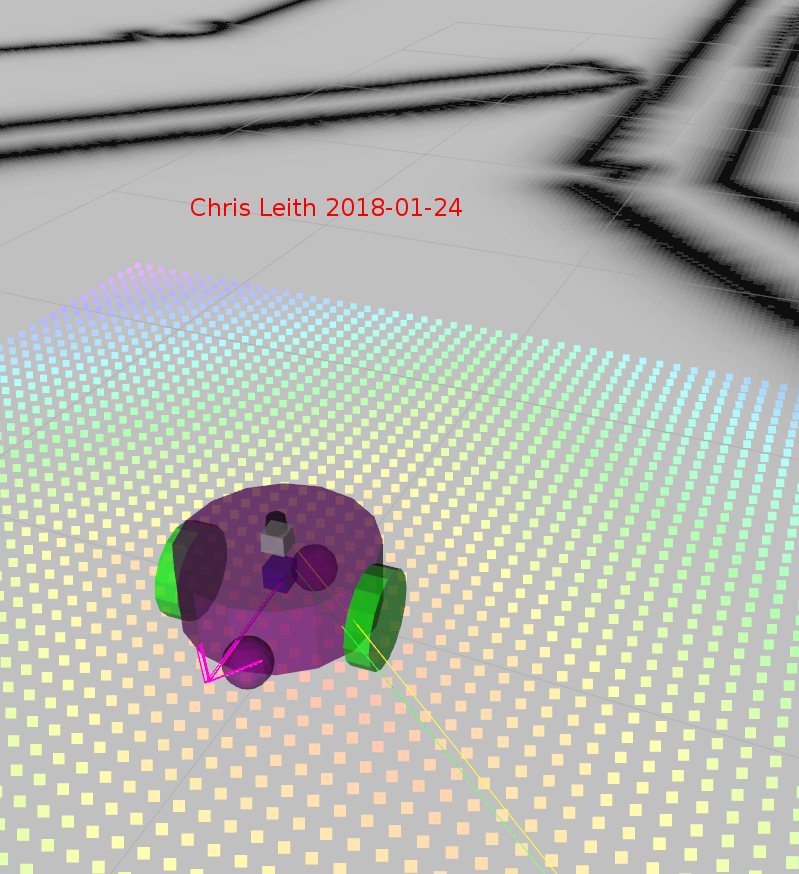
\includegraphics[width=\linewidth]{../Assets/writeupImages/cielBot_rvizGoal.png}
      \caption{cielBot Goal Particles }
      \label{fig:cielBot Goal Particles}
\end{figure}


\section{Model Configuration}
Tuning the parameters of the model was a time consuming and haphazard process, esecially in light of the sparse instructions provided and the terse documention available.
A minimum of guidance from the project description provided suggestions on how to proceed and various web resources including the ROS Navigation Tuning Guide and the udacity forums provided various tips on parameters of interest. With this nebulous set of tips I was able to slowly make progress on improving the behaviour of the robot. Following is a summary of some of the parameter modifications that were found to be helpful.

\subsection{Udacity-Bot}
The first runs of the bot generated many timeout errors - it seemed the processing load was too much for the laptop used, so ways to decrease the processing load were reviewed in the various resources listed above. The first thing change was to decrease the min and max particles drastically. In the final configuration successful navigation was obtained using a min of 10 particles and a max of just 50. Next was a decrease in the size and resolution local cost map seemed to help, although this was decreased even further later for other reasons. 
There were still some timeout warnings, which without clear guidance as to what processes were actually timing out led to decreasing numerous publishing and update frequencies: in costmap\_common global\_costmap and local\_costmap. Some timeouts continued but the bot was showing signs of navigating albeit in a jerky motion and very jerky map updates. Next up were the odom\_alphas 1-4. Setting larger than the default (0.2) seemed to create particle divergence. All were set to a very small value (0.005) compared to the default and this sped up paricle convergence. The inflation\_radius was increased to 0.7 and this caused the robot to give a clearance buffer around obstacles that decreased collisions. There were times when the robot would turn into the wall, especially near the hairpin turn. Decreasing the local cost map size even further ensured that the robot would not attempt a local 'shortcut' to the global path nearby on the the other side of the barrier. Increasing the pdist parameter also helped keep very close to the global path.

\subsection{Ciel-Bot}
Due to a shortage of time the custom robot, CielBot (udacity\_robot\_ciel in the project files) was designed only superficially different from the udacity bot. This permitted reuse of all of the parameters used by the udacity bot. Even this had some problems. Putting the laser in the middle of the chassis disk caused the laser to to scan the tops of the wheels. The dimensions of the wheels, casters and the disk all had to be redesigned to avoid this while also ensuring that the laser scanner remained perfectly horizontal. Otherwise this robot performed almost identically using the same costmap parameters.


\section{Discussion}
The results of the robot localization and navigation were satisfactory. However the haphazard trial and error approach of 'turning knobs' to see what happens may not be the most effective way to gain an understand of what the paramters do. This is due to the complexity of the system. If one parameter is badly tuned it may completely mask changes to other parameters. In particular it was a lengthy process to fix the jerky map and also the spinning problem and changing parameters in one sequence might appear to make no improvement while in another sequence the results problems would be fixed. This leaves one with a muddled sense of what all the parameters really do in pratice. However the process definitely enhanced understanding of ROS and AMCL and how powerful AMCL can be. It is clear that AMCL is a very practical technique to use in both local localization and with random particle augmentation in global localization. The kidnapped robot problem would not, in general be solvable with AMCL without further modification because the robot would have to recognize that even the highest weight particles of its converged solution were grossly in error. A possible solution is to characterize the particle weights for gross mis-loclization and then proceed to expand the number and dispersal of particles alhough on a very large map this may not work in practice. But for well defined environments such as a factory floor or a well mapped roadway systems and where odometry is reliable AMCL should be able to localize quite effecively. Porrly defined environments such as forests or rocky terrain with very few known landmarks would nearly impossible for AMCL to localize without assistance from another systems such as GPS or wifi or cell signal landmarks.

\section{Conclusion / Future work}
The project was a success both in terms of simple robot goal of designing a robot that uses AMCL in ROS/Gazebo to succusfully localize and navigate within its environment and in terms of the wider goal of gaining experience and incread understanding of AMCL and it's subleties and the ROS/Gazebo environment as a robot design and test platform. Future work could include integrating other sensors into the robot, eg IMUs, radar, ultrasonic rangers, GPS and more. Also using a more challenging map and more challenging goals like waypoint navigation around the entire map. And of course the real challenge will be to implement the whole design on a real robot running ROS in the real world. It would be great fun but surely many unexpected challenges would arise including many discreapancies between running ROS in the real world versus running ROS in the Gazebo environment. And lastly, the next projects will involve localization and mapping (SLAM) for the case where the world map in incompletely known or changing over time.

\end{document}